\documentclass[russian,utf8,a1paper,nostitching,simple]{eskdgraph}
\usepackage[T2A]{fontenc}
\usepackage{pscyr}
\usepackage{tikz}
\usepackage{color}

\newcommand{\No}{\textnumero}

\ESKDunitName{Реализация программного модуля}
\ESKDsignature{ГУИР.000000.002 ПЛ}
\ESKDletter{}{Т}{}
\ESKDauthor{Будный}
\ESKDchecker{Сальников}
\ESKDcolumnXIfIII{Лаппо}
\ESKDnormContr{Протченко}
\ESKDapprovedBy{Навроцкий}
\ESKDgroup{ИТАС, гр. 120602}

\renewcommand{\ESKDcolumnXfIVname}{Реценз.}
\ESKDcolumnXIfIV{}

\begin{document}

\ESKDthisStyle{empty}
\begin{ESKDdrawing}
  \centering
  {\fontsize{50}{60}\selectfont Реализация программного модуля}

  \vspace{2cm}
  % \hline
  \centering
  \ESKDfontX{Взаимодействие классов подсистем} \\
  \vspace{2cm}
  \centering
  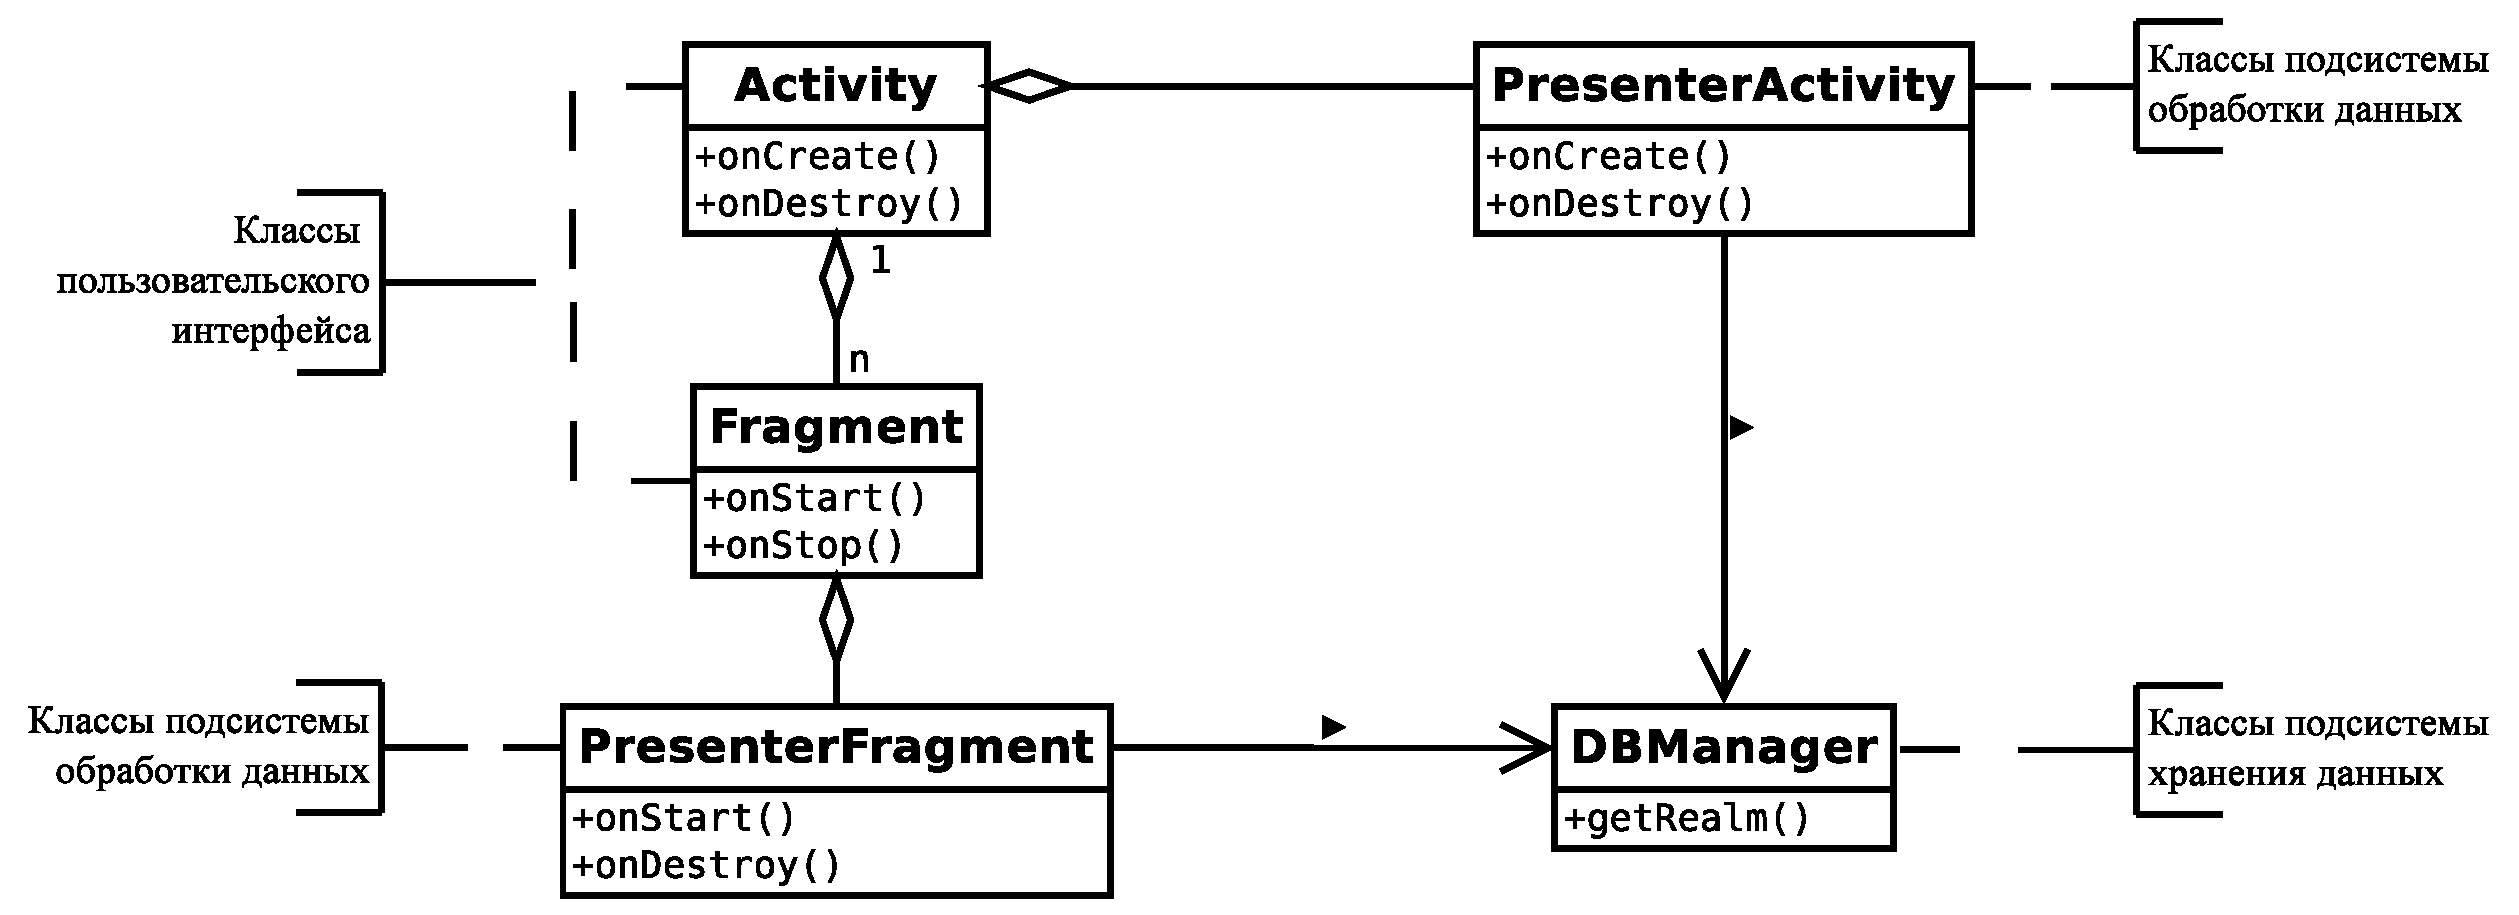
\includegraphics[height=24cm]{fig/implementation_bl_presenter_big.eps}


  \vspace{4cm}
  % \vline
  % \hline
  \begin{minipage}{50cm}
    \centering
    \ESKDfontX{Модель данных} \\
    \vspace{2cm}
    \centering
    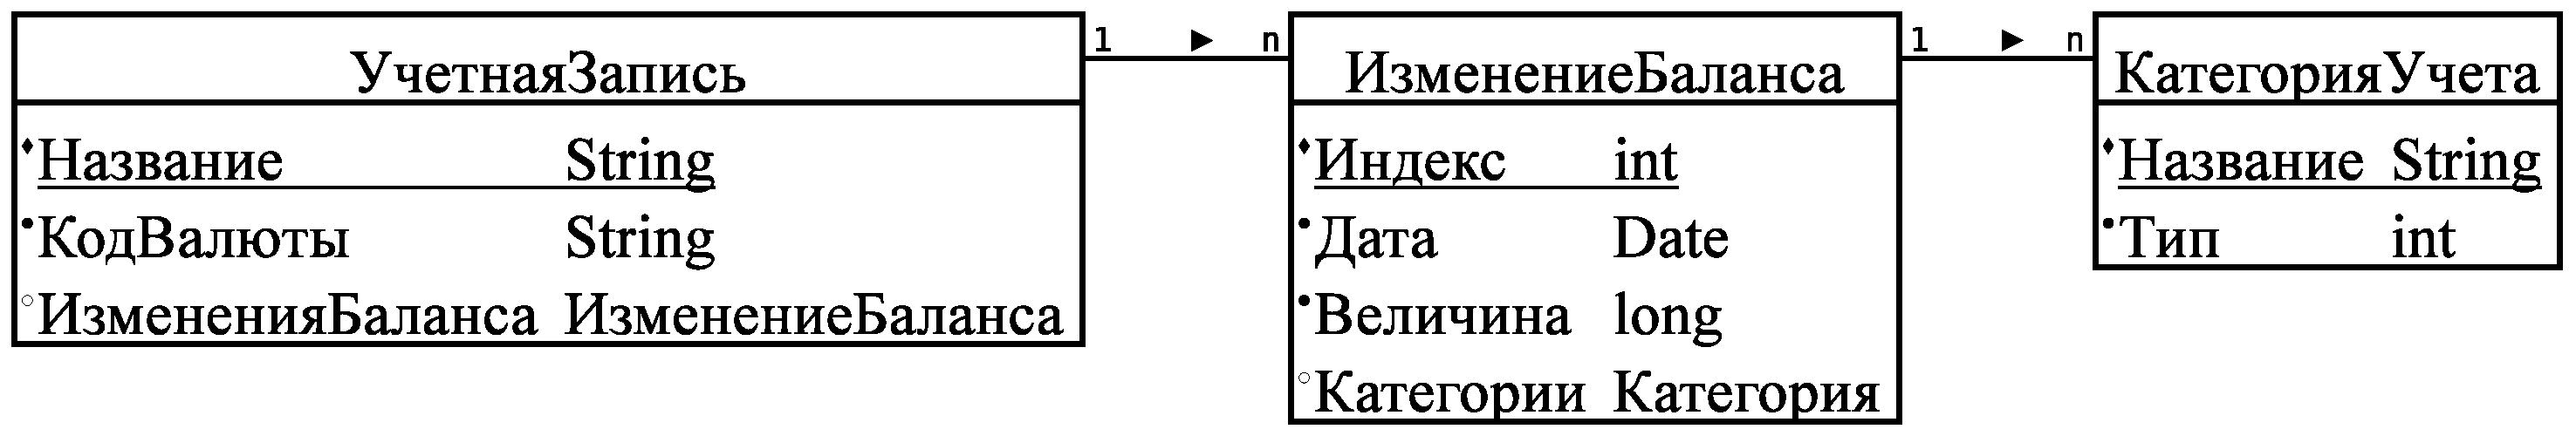
\includegraphics[width=50cm]{fig/design_entities.eps}
  \end{minipage}
  % \vline
  \hspace{2cm}
  % \vline
  \begin{minipage}{20cm}
    \centering
    \ESKDfontX{Иерархия классов подсистемы \\ обработки данных} \\
    \vspace{2cm}
    \centering
    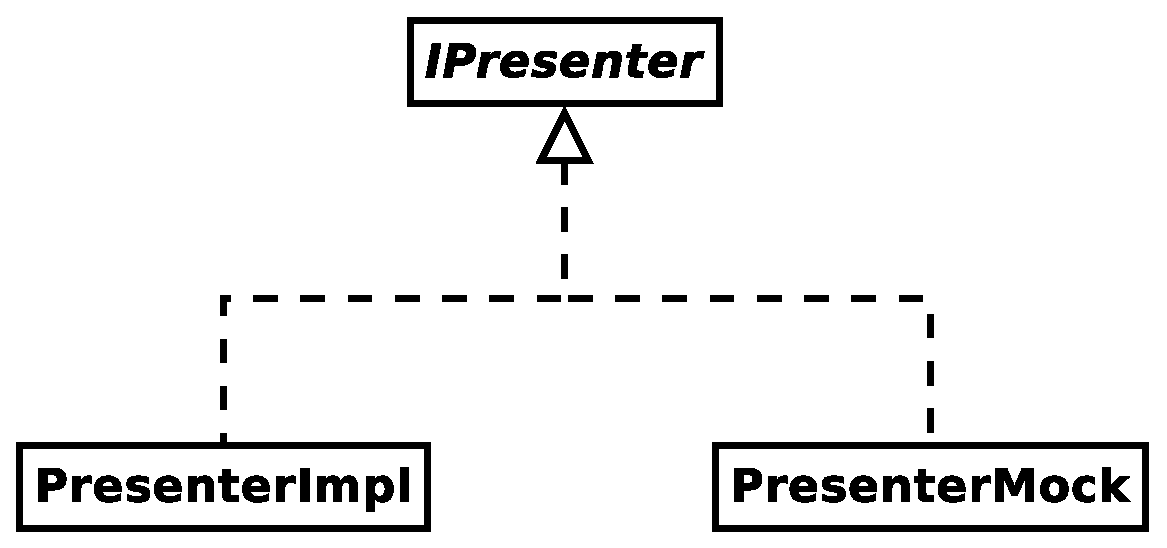
\includegraphics[width=20cm]{fig/implementation_testing_presenter.eps}
  \end{minipage}
  % \vline
  % \hline
\end{ESKDdrawing}

\setcounter{page}{1}
\ESKDthisStyle{formI}
\begin{ESKDdrawing}
\end{ESKDdrawing}

\end{document}
